\chapter{LITERATURE REVIEW}


\section{Parametric Representation of curves and surfaces}

The standard for describing and modeling curves and surfaces in computer aided design (CAD) and computer graphics is NURBS, or NonUniform Rational B-Splines. Extensive mathematical coverage describing NURBS are found in the seminal books of \cite{Rogers:2001} and, \cite{Piegl-etal:1997}. \\

Essentially, NURBS describe parametric curves and surfaces. Curves and surfaces are mathematically represented either explicitly, implicitly or parametrically. \\

In general, a parametric curve representation of a 3D curve takes the mathematical functional form of $C(x(u), y(u), z(u))$ where $x(u)$, $y(u)$, and $z(u)$ are mathematical functions in the independent parameter $u$, bounded by a range $u_{min}$ $\le$  $u$ $\le$ $u_{max}$.\\
 
By extension, a parametric surface representation of a 3D surface takes the form of $S(x(u,w), y(u,w), z(u,w))$ where $x(u,w)$, $y(u,w)$, and $z(u,w)$ are mathematical functions in two independent parameters $u$ and $w$. The parameters $u$ and $w$ must also be bounded.\\
 
When compared to either explicit or implicit formulations, this parametric representation is extremely flexible. The representation is axis independent, easily represented by multiple-valued functions and, can have infinite derivatives. Furthermore, to have more degrees of freedom independent parameters can be added.\\

In practice, curves and surfaces are generally bounded. When either an explicit or implicit representation is used, imposing the boundaries is awkward. In contrast, the boundaries for a parametrically represented curve or surface are provided by the restrictive parameter ranges. In addition, the parameter range for a parametric curve also specifies a natural traversal direction along the curve. \\

As an example, for a 3-dimensional curve with independent parameter $u$ in the range $u_{min}$ $\le$  $u$ $\le$ $u_{max}$, the curve direction will be from the point $C(x(u_{min}), y(u_{min}), h(u_{min}))$ to $C(x(u_{max}), y(u_{max}), h(u_{max}))$ as $u$ increases from $u_{min}$ to $u_{max}$.\\

Note that specifying a curve requires one parameter while a surface requires two parameters. Also a parametric curve with the function $h(u)$ being zero for all values of parameter $u$ means the curve is 2-dimensional or a curve in the x-y plane.


\section{Continuity of curves and surfaces}

There are two kinds of continuity, or smoothness, associated with parametric curves and surfaces known as geometric continuity $G^{n}$, and parametric continuity $C^{n}$, where $n$ is the order of the derivative. Simplistically, you can think of geometric continuity as physical and parametric continuity as mathematical. Geometric continuity is less restrictive than parametric continuity. This means that if it is $C^{n}$ continuous, then it implies $G^{n}$ continuous, but not the opposite. The fundamental difference between geometric $G^{n}$ and parametric continuity $C^{n}$ can be illustrated as follows. \\

Given a parametric vector-valued function, $P(u)$, over some parameter range $u$ describing a curve, then any given value of $u$ represents a specific point on the curve. The first derivative, $P^{'}(u)$, represents the velocity of a point as it moves along the curve, and the second derivative $P^{''}(u)$ represents the acceleration. \\

If the curve is $C^{1}$ continuous at a join, then both the direction and magnitude of the tangent vector are equal across the join; and the point smoothly transitions from one curve segment to the next. If, however, the curve is only $G^{1}$ continuous at the join, then as the point transitions across the join the direction of motion does not change (tangent vector direction), but there is an instantaneous change in speed (tangent vector magnitude) that represents an instantaneous acceleration as the point transitions across the join. If the curve represents a path trajectory for a CNC machine, the abrupt velocity (magnitude) change will cause a sudden jerk.\\

Note that $C^{0}$ means the parametric continuity of the curve itself, and $C^{1}$ and $C^{2}$, the continuity of its first and second derivatives, respectively. All of the parametric curves selected and used in this work are $C^{2}$ continuous.

%% =======================================================
\clearpage
\pagebreak
\section{Computerized Numerical Control (CNC) Systems}

A typical machine architecture for a 3D-four-axis machine is shown in Fig [\ref{CNC-Basic-Architecture.png}]. The 3D axes corresponds to the x, y, and z motion axes while the fourth is the rotating axis of the spindle cutting tool. Fig [\ref{CNC-Servo-and-Spindle-Driving-Mechanism.png}] shows the mechanism of the axial motions and the rotational motion of the spindle while Fig [\ref{CNC-Typical-Software-Control-Flow-Diagram.png}] shows the typical software control flow diagram for a typical CNC machine.\\


CNC manufacturing operations involve the generation of reference signals describing the geometrical parts to be machined and the control of the machine such that it follows those reference signals. In modern CNC machines, the generation of reference signals, construction and execution of control loops are accomplished in software within a computer. Fig [\ref{Functional-Architecture-of-CNC-System.png}] shows the block diagram for the functional architecture of a typical CNC system.\\

%% \noindent
A modern commercial CNC 3D-four(4)-axis milling machine is shown in Fig [\ref{CNC-Commercial-Milling-Machine.png}]. The fourth axis is the rotational axis for the spindle cutting tool. An example of a a commercial CNC lathe machine is shown in Fig [\ref{CNC-Commercial-Lathe-Machine.png}]. Modern commercial CNC machines today have extended milling and turning to 9-axes, for example, the DN Solutions PUMA SMX3100ST combined milling and turning machine. \cite{TitanCNC:2021} shows a YouTube video of this 9-axes CNC in action.\\


\begin{figure} 
	%%	\centering
	\caption{Basic achitecture for a typical CNC system}
	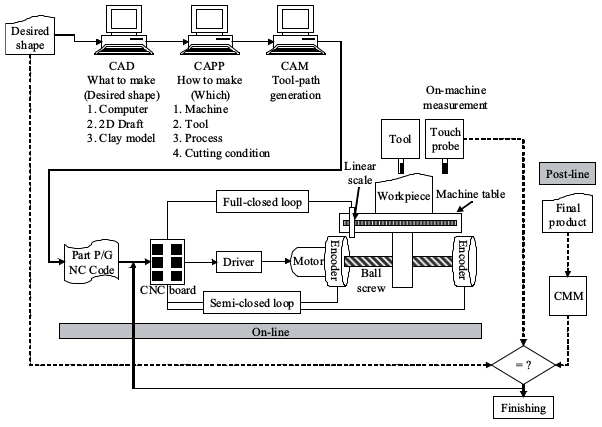
\includegraphics[width=0.90\textwidth]{Chap2/Images/CNC-Basic-Architecture.png} 
	\label{CNC-Basic-Architecture.png}
\end{figure}

%% ==========================================
\clearpage
\pagebreak

\begin{figure}
	%%	\centering
	\caption{Typical Servo drive and spindle driving mechanism}
	\label{CNC-Servo-and-Spindle-Driving-Mechanism.png}
	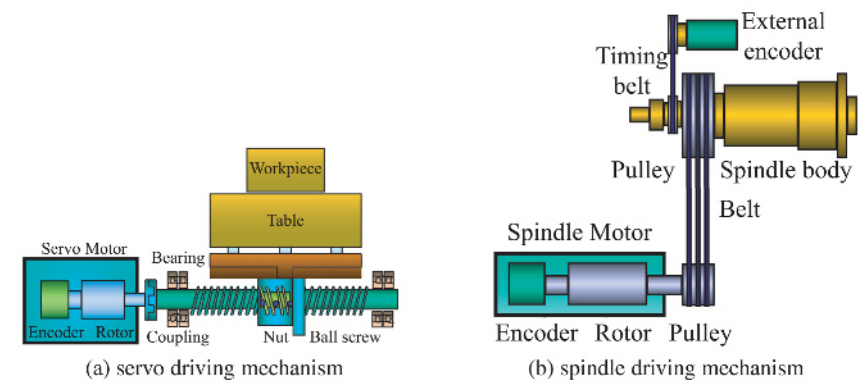
\includegraphics[width=1.00\textwidth]{Chap2/Images/CNC-Servo-and-Spindle-Driving-Mechanism.png} 
\end{figure}



\begin{figure}
	%%	\centering
	\caption{Typical CNC Software control flow diagram}
    \label{CNC-Typical-Software-Control-Flow-Diagram.png}	
	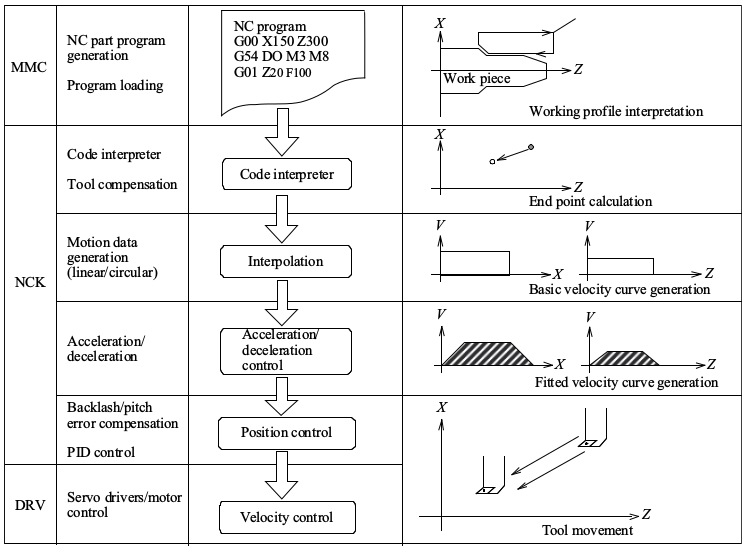
\includegraphics[width=1.00\textwidth]{Chap2/Images/CNC-Typical-Software-Control-Flow-Diagram.png} 
\end{figure}

\clearpage
\pagebreak

\begin{figure}
	\centering
	\caption{Typical CNC Functional Architecture}
	\label{Functional-Architecture-of-CNC-System.png}
	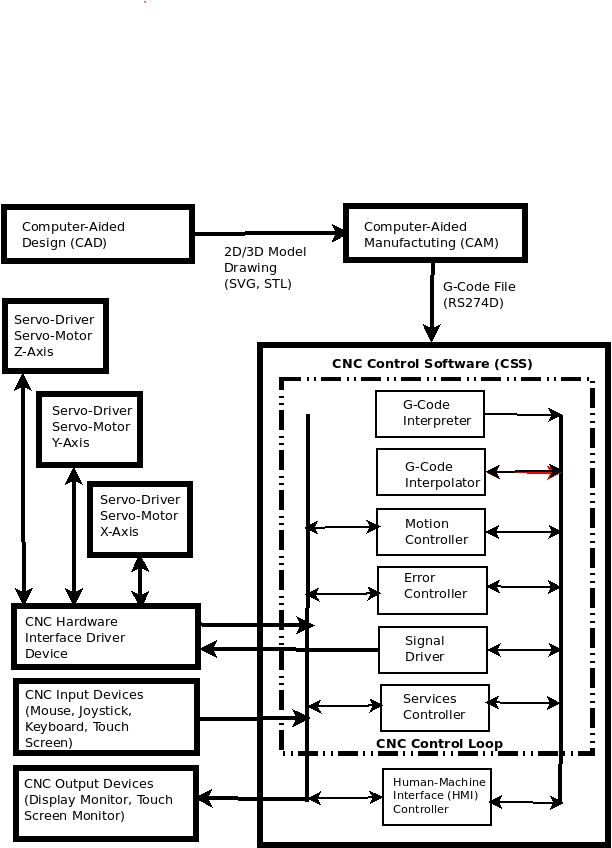
\includegraphics[width=1.00\textwidth]{Chap2/Images/Functional-Architecture-of-CNC-System.png} 

\end{figure}


\clearpage
\pagebreak
\begin{figure}
	\centering
	\caption{Typical CNC Commercial Milling machine}
    \label{CNC-Commercial-Milling-Machine.png}	
	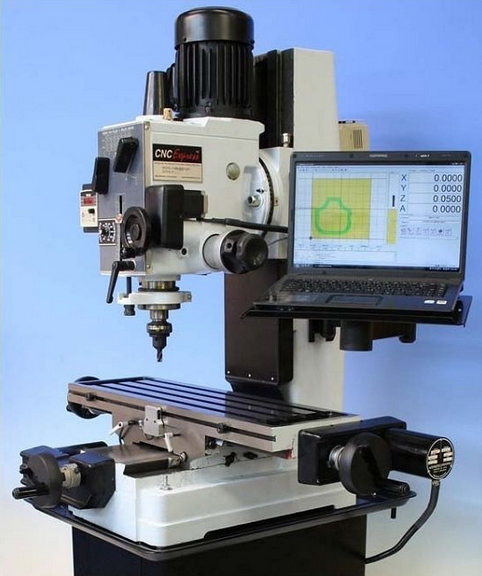
\includegraphics[width=1.00\textwidth]{Chap2/Images/CNC-Commercial-Milling-Machine.png} 
\end{figure}

\clearpage
\pagebreak
\begin{landscape}
\begin{figure}
	\centering
	\caption{Typical CNC Commercial Lathe machine}
    \label{CNC-Commercial-Lathe-Machine.png}	
	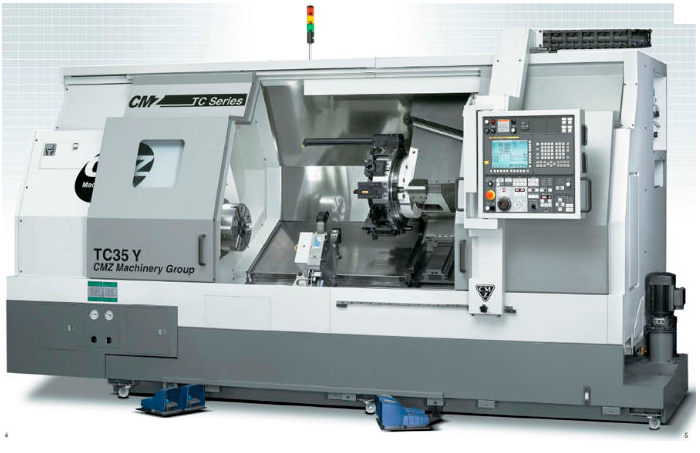
\includegraphics[width=1.40\textwidth]{Chap2/Images/CNC-Commercial-Lathe-Machine.png} 
\end{figure}
\end{landscape}



%% ===========================================================
\clearpage
\pagebreak
\section{Advantages of Parametric Representations in CNC}

Parametric interpolation has many merits over the traditional linear (G01) and circular interpolation (G02 and G03) in terms of model representation, feedrate smoothness and application range. \cite{Jin-etal:2014} reported some advantages below.\\

\begin{enumerate}
	\item In parametric interpolation, the geometrical information of the machining paths can be totally as well as accurately transferred to the CNC systems without any approximation errors and data loss. This error and loss may occur in conventional linear and circular interpolation.
	
	\item The parametric interpolator code only needs some critical parameters of the machining contours (i.e. control points, knot vectors, weights as in NURBS). Such a transmission mechanism can guarantee the efficiency of interaction between the host and slave machines.
	
	\item In parametric interpolation, feedrate continuity and smoothness are achieved effectively since the joints between tiny segments do not require repeated acceleration–deceleration processes. In traditional interpolation methods repeated acceleration–deceleration may not be avoidable.
	
	\item Parametric interpolation is still possible in conventional CNC systems after some developments of the machining parts. This may include approximating tiny parts into curve segments and optimization with parametric curves between them.
\end{enumerate}

%% ======================
\clearpage
\pagebreak

\section{Interpolation of parametric curves}

The problem statement for interpolation of a parametric curve is: \\

\textit{Given the parametric curve $C(u)$, determine $u(k)$ for the $k_{th}$ interpolation period, the re-parametrization of $u$ with time $t$ is required, that is, solve the function $u = u(t)$, where $u$ is the independent parameter, and $t$ is time.}\\

In other words, it means at a point on the parametric curve $C(u)$, find the next $u$ point. The next $u$ point is a function of time $t$.\\

Since the machine moves with time, the re-parametrization from $t$ to $u$ should be subjected to the machine dynamic constraints and contour error tolerance. It can be described as follows. 

\begin{enumerate}

\item The machine axial velocities and accelerations should be limited to avoid saturating the axes. These are the first and second derivatives of the corresponding parametric function $C^{'}(u)$ and $C^{''}(u)$ with $u = u(t)$, over time, respectively. 

\item The limitations include satisfying specific machine characteristics like startup torque, maximum and minimum velocity (feedrate), maximum and minimum acceleration (jerk), and encoder resolution (incremental motion stepping). 

\item In order to guarantee a smooth trajectory motion profile the jerk should be limited or completely eliminated. This ensures a smooth feedrate profile.  

\item The contour error $\epsilon$ increases with increasing feedrate, so the feedrate should be limited to achieve high contour accuracy. There should be an optimum strategy to balance contour error and machine feedrate.

\end{enumerate}

The function of the real-time interpolator in a computer numerical control (CNC) machine is to compute a reference point in each sampling time interval T (for example, 0.001 s), of the servo system, based on a prescribed tool path (curve) and feedrate data. \\

By comparing the actual instantaneous machine position (measured by encoders on the machine axes) with the reference point, accurate closed-loop control of the machine position and speed may be obtained.\\




%% ======================
\clearpage
\pagebreak

\section{Previous works on parametric interpolation}


Probably, \cite{Koren:1976} was the first to introduce the general concept of interpolation for a {CNC} system.  Later, \cite{Koren-etal:1993} and \cite{Shpitalni-etal:1994} extended the idea to basic approximation principles for parametric curves. \\

The two common technical routes that have been developed for the interpolation of parametric curves are the arc length parametrization and the recursive/iterative Taylor's expansion. \\

It was reported by \cite{Farouki-etal:2001} that near arc length parametrization is possible with some numerical methods. However, it is computationally intensive with the approximation error accumulating along the curve. This especially occurs in curves with large curvature variations like sharp turns, and with uneven parameter computations.\\

In order to realize parametric interpolation, researchers developed a wide variety of methods to achieve better machining qualities. The common adopted approaches for interpolating parametric curves were based on Taylor’s expansion, for example, \cite{Cheng-etal:2002}.\\

\cite{Farouki:2021} considered realtime interpolators based on Taylor series to possess two inherent shortcomings. Firstly, the occurrence of truncation errors because only a finite (small) number of terms can be employed, and secondly, for variable feedrates, the coefficients of higher-order terms, defined by successive chain-rule differentiation, become increasingly complex and cumbersome, especially when involving computationally intensive expressions.\\

A parametric interpolation method based on prediction and iterative compensation was proposed by \cite{Ni-etal:2019} where the feedrate fluctuation and Taylor’s expansion were analyzed to reduce the calculation accuracy of truncation errors caused by neglecting the high-order terms. \\

Another method for parametric interpolation is named 'guide curve based'. It was developed by \cite{Sun-etal:2006}. This method implements the near arc length parameterization. Essentially, the detection of corners and key regions are done offline, and this approach schedules feedrate based on a guide curve without a look-ahead facility. \\ 

\clearpage
\pagebreak


Although available CNC interpolators for parametric curves generally achieve contouring position accuracy, the specified feedrate, which dominates the quality of the machining process, is not guaranteed to be smooth during motion. Severe speed fluctuations may incur tool chatter or breakage, especially in high speed machining. Since feedrate control is crucial, \cite{Yeh-etal:1999} for example, developed a speed-controlled interpolator for machining parametric curves. \\

Later, \cite{Yeh-etal:2002} considered interpolation of parametric curves by adapting the feedrate with a confined chord error while  \cite{Nam-etal:2004} proposed an approach for parametric interpolation that allows the feedrate profile to be dynamically adjusted according to geometrical path constraints. \\

Tracking error and contour error are two very important aspects that need to be effectively handled by any CNC servo control system.  \cite{Ramesh-etal:2005} reviewed the various techniques that have been developed in minimizing and eliminating tracking and contour errors.\\ 

A much later review, 13 years after, was conducted by \cite{Jia-etal:2018} on the subject of contouring-error reduction method in multi-axis CNC machining. The review covers both three-axis and five-axis contouring-error reduction methods. The methods comprise various offline contouring-error reduction, interpolator designs for contouring-error reduction, cross-coupling schemes for direct contour control and contour control algorithms. As an example, \cite{Chen-etal:2019} considered contour error-bounded parametric interpolator with minimum feedrate fluctuation. \\

The paper by \cite {Lee-etal:2018} reviews recent progress of control technologies for precision machining using CNC in the area of interpolation, contour control and compensation. In terms of interpolation several corner blending methods and parametric curves are introduced and the characteristics of each method discussed. In addition, contour control algorithms recently developed for multi-axis machines are also reviewed.\\

In another direction, \cite{Bhattacharjee:2012}, instead of using Taylor's expansion approximation, employed the classical fourth-order Runge-Kutta (RK) method using only the first derivative to generate successive parameter values for the calculation of x, y, z coordinates of interpolated points. It was done in order to avoid calculating higher derivatives and make the interpolation calculations simpler.\\

\clearpage
\pagebreak

On parallel implementation, \cite{Fu:2016} developed a parallel CNC system architecture based on Symmetric Multi-Processor (SMP). This  subject is of interest to this author. The author's involvement on parallelism in CNC is discussed in the next section, where FPGA (Field Programmable Gate Arrays) programming was used to drive the CNC machine.\\


\section{Related CNC work by the author}

Low end research CNC machines, like the CNC UMP Model 2008 in Fig [\ref{chap2-CNC-Research-Machine-3-Axis.jpg}], can be controlled and driven using small devices and (IoT) gadgets, like desktops, laptops, computer extension boards and single-board-computers (SBC).\\ 

\cite{Kalimbetov:2012} used C/C++ and Python codes on a Linux box driving the UMP CNC model 2008 machine in realtime using a customized parallel port software driver. Comparisons were conducted running the CNC on both realtime (RTOS) and non-realtime (NRTOS) operating systems. \\

\cite{Ariffin:2014} used the USB based Arduino Due extension board to drive the UMP CNC machine. This resource limited hardware (only 512 KB onboard user Flash memory) required a special technique in writing the C/C++ codes for the CNC software driver.\\  

\cite{Abdelgader:2014} used a combination of gadgets to drive the CNC machine, using the computer laptop, the proprietary Heber X10i extension board and the Raspberry Pi 2 single board computer (SBC). The Raspberry Pi a low cost, credit-card sized, full board computer was successfully used to drive the CNC machine. Since, the memory addresses of the driving pins in the Heber X10i hardware are separated, a special technique was developed to get the memory register addresses contiguous. \\

\cite{Ahmad:2017} later used the Raspberry Pi 3 Model B, an updated version to drive a CNC machine in Real Time. An output for this work is shown in Fig [\ref{Thank-You-WRY-Asyrul.png}]. The step by step CNC process from start to finish (capture image, convert image to G-code, drive G-code on UMP CNC machine) executed by \cite{Ahmad:2017} is shown in an interesting video accessible at the link: [\href{https://www.youtube.com/watch?v=4s94wy6ZGJE}{CNC Rpi3 Real Time, 5m:46s}]. The video is demonstrated with a beautiful background rendition of the song "Jalur Gemilang", a snapshot of it is provided in [\ref{chap2-CNC-Jalur-Gemilang-Rendition-Video.png}].

\clearpage
\pagebreak

\cite{Selvarajah:2015} deployed the Beagle Board xM single board computer (SBC), to drive the CNC machine. This Beagle Board xM is a variation of SBC gadgets with more capabilities than the Raspberry PI. This board used the OMAP (Open Multimedia Applications Platform) processor, which is capable of video and image processing. OMAP is mostly used in commercial cell phones.\\ 

The highlight is the work of \cite{Teh:2016} that engaged the Nexys-3 Spartan-6 FPGA board to develop a closed-loop feedback system that controlled the CNC machine. An image of this quite expensive board is provided in Fig [\ref{Nexsys3-Spartan6-Xilinc-board.jpg}] at the bottom right. the green board with a USB-UART connection. \\

FPGAs are truly parallel in nature, so different processing operations do not have to compete for the same resources. In addition, the inherent parallel execution of FPGAs allows for independent pieces of hardware logic to be driven by different clocks. Depending on design, FPGA processors execute multiple tasks at any one time. This is unlike typical Intel x86 or ARM processors that execute line by line.\\

FPGAs are powerful pieces of technology that allow users to implement custom hardware (not software) designs. There are several FPGA programming languages available, but the four most popular are VHDL, Verilog, SystemVerilog, and C/C++. \\

This project utilized a mixed of VHDL and C/C++ languages to program the Nexys-3 hardware that generated the CNC driver codes on the the board. A G-code file on the computer was first converted to a signal file, reference Fig [\ref{Gcode-left-to-Nexys3-signal-file-right.jpg}]. Then, the file is transmitted from the computer to the Nexys-3 board via USB-UART serial protocol. The received signals are then sent by the Nexys hardware to the three(3) x, y, z axial motors of the CNC machine, with the three tasks running parallel in time. Since parallel execution is natural to FPGA operation, the project goal of true parallelism was achieved.\\

Real live Youtube videos of successful CNC executions can be accessed at the following links:  
[\href{https://www.youtube.com/watch?v=3GuhE5dlcYk}{CNC FPGA-Video1, 0:56s}], 
[\href{https://www.youtube.com/watch?v=VvAyLqt\_wLQ}{CNC FPGA-Video2, 0:58s}] and 
[\href{https://www.youtube.com/watch?v=gvlKlqfEXro}{CNC FPGA-Video3, 4m:00s}]. \\

The acquired detailed knowledge, skills and understanding of these diverse raw hardware and their environments, as mentioned in the projects above, is critical to the success of the present author's thesis.\\ 

%% ==================================
\clearpage
\pagebreak

\begin{figure}
	\caption{ CNC UMP Model 2008 - University Malaysia Pahang}
    \label{chap2-CNC-Research-Machine-3-Axis.jpg}
	\centering
	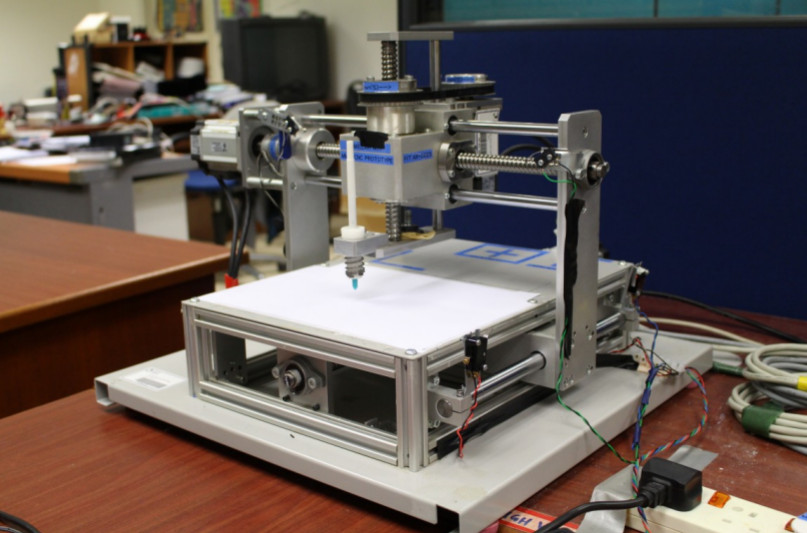
\includegraphics[width=0.95\textwidth]{Images/Chap4/CNC/CNC-Research-Machine-3-Axis.jpg} 
\end{figure}


\begin{figure}
	\caption{Youtube: CNC Jalur Gemilang Rendition Video by Ahmad (2017)}
	\label{chap2-CNC-Jalur-Gemilang-Rendition-Video.png}
	\centering
	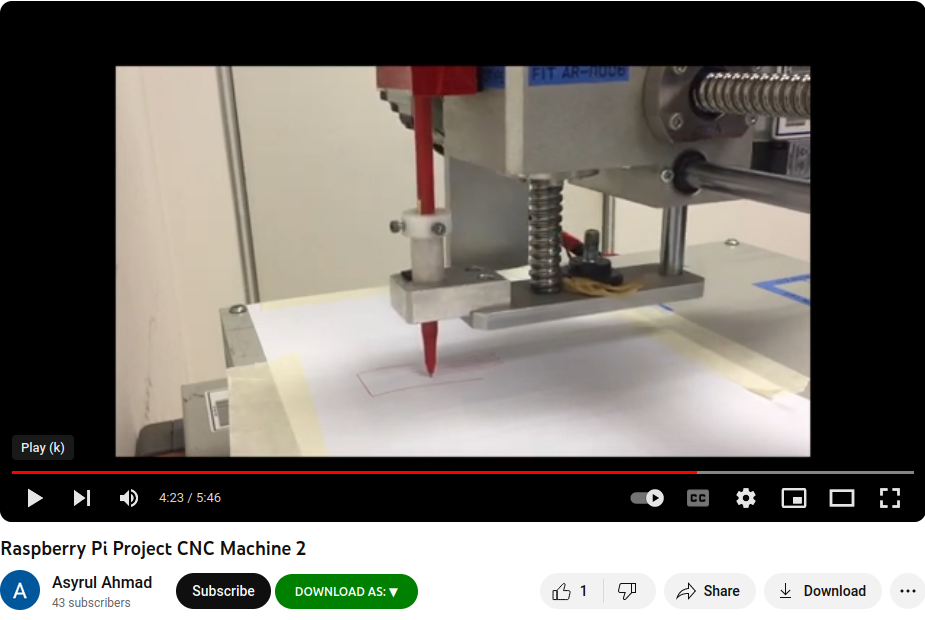
\includegraphics[width=0.95\textwidth]{Images/Chap3/CNC-Jalur-Gemilang-Rendition-Video.png} 
\end{figure}

%% ===================================
\clearpage
\pagebreak

\begin{figure}
	\caption{Proton logo output of UMP CNC machine by Ahmad:2017}
	\label{Thank-You-WRY-Asyrul.png}
	\centering
	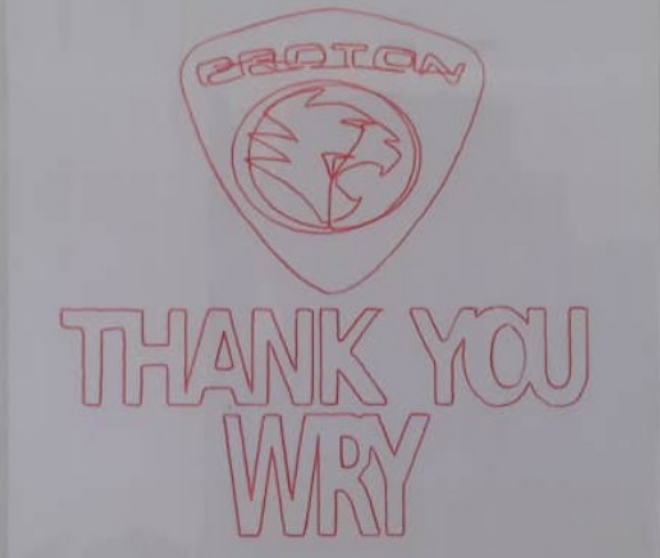
\includegraphics[width=0.95\textwidth]{Chap2/Images/Thank-You-WRY-Asyrul.png} 
\end{figure}

\begin{figure}
	\caption{Setup of Nexsys-3 Spartan-6 Xilinc board by Teh:2016}
	\label{Nexsys3-Spartan6-Xilinc-board.jpg}
	\centering
	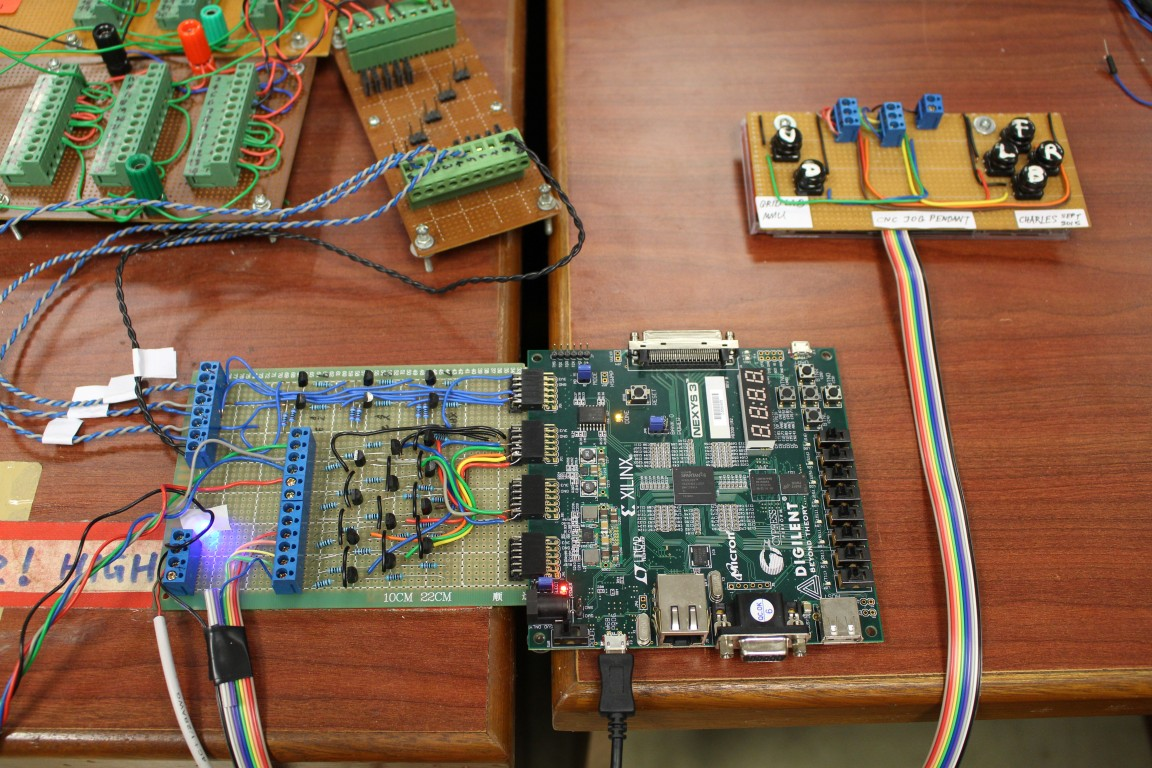
\includegraphics[width=0.95\textwidth]{Chap2/Images/Nexsys3-Spartan6-Xilinc-board.jpg} 
\end{figure}

%% ======================
\clearpage
\pagebreak

\section{Comparisons previous works with this thesis}

Previous works had definitely looked into the issues of chord-error and feedrate in parametric curve interpolations, but in a different perspective compared to the work in this thesis. \\

The early paper by \cite{Yeh-etal:1999} formulated real-time CNC interpolators for variable feedrates along parametric curves. Later, \cite{Farouki-etal:2001} pointed an erroneous coefficient for the quadratic term in the paper. \\

It was mentioned by \cite{Farouki-etal:2001} that, Pythagorean-hodograph (PH) curves admit closed-form analytic reductions of the interpolation integral, yielding real-time interpolators that are essentially exact, and remarkably versatile in terms of the repertoire of feedrate variations (with time, arc length, or curvature) they accommodate. The work in this thesis, also involves feedrate variations with time, arc length, and curvature however, it does not involve Pythagorean-hodograph (PH) curves. \\

\cite{Farouki:2021} considered the successive applications of the differentiation chain rule which are necessary to determine Taylor series coefficients beyond the linear term as being cumbersome, so the use of Richardson extrapolation as a simple means to compute rapidly convergent approximations to the higher-order coefficients was introduced. The work in this thesis, however, does not involve Richardson extrapolation. \\

The work by \cite{Jin-etal:2014} breaks parametric interpolation into rough interpolation and fine interpolation. According to \cite{Jin-etal:2014}, rough interpolation is about feedrate adjustments between two successive interpolation periods, while fine interpolation is about adjusting the feedrate to comply with the geometrical constraints and kinematical characteristics of the CNC machine. The work in this thesis however, implements feedrate adjustments immediately in one interpolation period taking into account of both  geometrical and kinematical constraints simultaneously. \\

The work by \cite{Zhong-etal:2018} does not impose an upper or lower limit for the chord-error. The values of chord-error are considered as whatever resulting from the algorithm running at the particular feedrate. In addition, \cite{Zhong-etal:2018} also allows for feedrate speedup to the value of command feedrate, for example, when it forsees a near straight line coming ahead, and this breaks the absolute feedrate limit constraint. 

\clearpage
\pagebreak

As a comparison, the work in this thesis imposes an upper limit for the chord-error, and strictly preserves both the chord-error and feedrate limit constraints at every point on the curve path, simultaneously. In addition, for feedrate smoothness throughout the entire traversal of the curve path, this thesis imposes a strict condition that does not allow acceleration jitters. This was not a condition mentioned in previous cited works. 


%% ======================
%% \clearpage
%% \pagebreak

\section{NURBS and G-Code programming}

NURBS are a type of spline, which is a curve or surface defined by a set of control points and a basis function. Unlike other splines, NURBS can have rational weights associated with each control point, which allow them to represent conic sections and other shapes that are not possible with polynomial splines. NURBS also have the advantage of being invariant under affine transformations, such as scaling, rotation, and translation, which makes them easier to manipulate and transform. NURBS can also be used to approximate any shape with arbitrary precision, by adjusting the number and position of the control points and the degree of the basis function. Reference: \cite{CollabCNC:2023A}\\

One of the main challenges of using NURBS in CNC programming is the compatibility and interoperability between different software and hardware systems. Not all CAD/CAM software can export or import NURBS data, and not all CNC machines can process or interpret NURBS data. Therefore, you may need to use different formats, standards, or protocols to exchange NURBS data between different platforms, such as IGES, STEP, DXF, or G-code. Another challenge is the quality control and verification of the NURBS data and the machined parts. You may need to use special tools or methods to check the accuracy, smoothness, and consistency of the NURBS data and the output, such as error analysis, simulation, or inspection. \cite{CollabCNC:2023B} discusses how to evaluate the accuracy and quality of NURBS machining results.\\

Low end CAD/CAM systems do not generate NURBS G-Code. However, NURBS have been used by high end systems CAD systems for some time. That is the main reason why it is natural that CNCs should be able to employ tool paths that are also defined in terms of NURBS.\\

This work covers only RS274D NGC G-Code files because the format is the base standard for G-Codes supported by all machines used in the CNC industry. This work does not include Scalar Vector Graphics (SVG) or STereoLithography (STL) files generated by CAD applications. It also excludes the generation of G-Codes from CAM processing of SVG or STL input files.\\

Using NURBS interpolation requires a CNC machine capable of handling NURBS G-Code generated tool paths. Since the NURBS G-Code format is proprietary and only used in the high end FANUC CNC machines. It should be noted that NURBS G-Code files are not the same as NURBS interpolation method. \cite{CollabCNC:2023A}, for example, discusses on how to integrate NURBS with other CNC programming methods and techniques.\\ 

Very recently, as of July 17, 2023, \cite {Hu-etal:2023} published a method for calculating interpolation points of NURBS curves based on chord length-parameter ratio. \\

The construction and manipulation of NURBS geometries is based on a structure with the following fields:
\singlespacing
\noindent
(1) number: the number of control points.\\
(2) coefs: control points coordinates (for NURBS also the weights).\\
(3) order: the degree plus one.\\
(4) knots: the knot vector in each direction

\section{Programming Languages for NURBS}

Traditionally, NURBS algorithms were developed using compiled C and C++ programming languages which are tedious and complicated to setup and use. It is available at the link [\href{https://www.nar-associates.com/nurbs/c_code.html}{C-Codes for NURBS}]. \\

\cite{Bingol-etal:2018} developed the \textit{NURBS-Python} library, a scripted, object-oriented, open-source pure Python library without external dependencies. This open-source library availability provides access for researchers to develop NURBS applications. It is provided at the link [\href{https://nurbs-python.readthedocs.io/en/5.x/}{Python-NURBS Website}] \\

Julia NURBS code is provided at the link [\href{https://github.com/eOnofri04/NURBS.jl}{Julia NURBS library at Github}] since Feb 20, 2019. Octave-NURBS is a collection of routines for the creation, and manipulation of Non-Uniform Rational B-Splines (NURBS), the latest release was on 2021-03-29. It is provided at link [\href{https://gnu-octave.github.io/packages/nurbs/}{Octave NURBS Website}]. \\

Note that, NURBS G-Code will not be in the scope of this research.  In this thesis, to drive the CNC machine, the approach is to adopt the second-order approximations of Taylor’s expansion, in an algorithm where the feedrate is calculated based on the value of chord-error and machine dynamic variables. The end objective is to constrain both chord-error and feedrate. For each point on the curve, the interpolation algorithm is computed in an iterative and recursive manner, back and forth, until it reaches a specified convergence criteria. \\

The interpolation algorithm in this work also generates a RS274D/NGC G-Code for each curve that later can be simulated offline, or executed directly on the UMP CNC machine to verify its success. 


%% ==============================================
\clearpage
\pagebreak
\begin{landscape}

\begin{figure}
	\caption{G-code file (left) and Signal file (right) for FPGA by Teh:2016}
	\label{Gcode-left-to-Nexys3-signal-file-right.jpg}
	\centering
	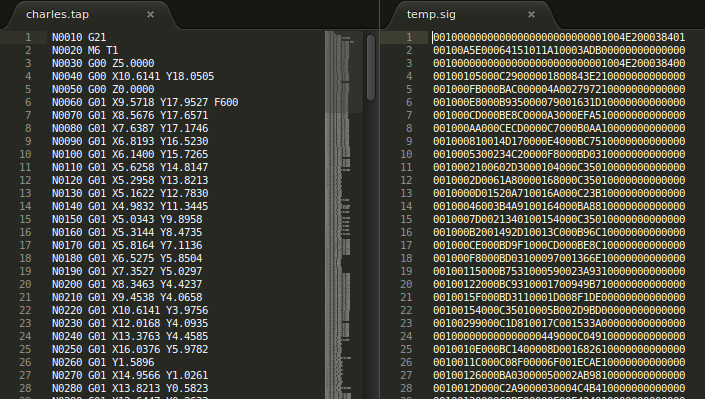
\includegraphics[width=1.62\textwidth]{Chap2/Images/Gcode-left-to-Nexys3-signal-file-right.jpg} 
\end{figure}

\end{landscape}